\documentclass[unicode,11pt,a4paper,oneside,numbers=endperiod,openany]{scrartcl}
\usepackage{amsmath}
\usepackage{float}  % To prevent floating of figures
\usepackage{lmodern}
\usepackage{listings}

\usepackage{ifthen}
\usepackage[utf8]{inputenc}
\usepackage{graphics}
\usepackage{graphicx}
\usepackage{hyperref}

\pagestyle{plain}
\voffset -5mm
\oddsidemargin  0mm
\evensidemargin -11mm
\marginparwidth 2cm
\marginparsep 0pt
\topmargin 0mm
\headheight 0pt
\headsep 0pt
\topskip 0pt        
\textheight 255mm
\textwidth 165mm

\newcommand{\duedate} {}
\newcommand{\setduedate}[1]{%
\renewcommand\duedate {See iCorsi for due date}}
\newcommand\isassignment {false}
\newcommand{\setassignment}{\renewcommand\isassignment {true}}
\newcommand{\ifassignment}[1]{\ifthenelse{\boolean{\isassignment}}{#1}{}}
\newcommand{\ifnotassignment}[1]{\ifthenelse{\boolean{\isassignment}}{}{#1}}

\newcommand{\assignmentpolicy}{
\begin{table}[h]
\begin{center}
\scalebox{0.8} {%
\begin{tabular}{|p{0.02cm}p{16cm}|}
\hline
&\\
\multicolumn{2}{|c|}{\Large\textbf{HPC Lab ---  Submission Instructions}}\\
\multicolumn{2}{|c|}{\large\textbf{(Please, notice that following instructions are mandatory: }}\\
\multicolumn{2}{|c|}{\large\textbf{submissions that don't comply with, won't be considered)}}\\
&\\
\textbullet & Assignments must be submitted to \href{https://www.icorsi.ch}{iCorsi} (i.e. in electronic format).\\
\textbullet & Provide both executable package and sources (e.g. C/C++ files, Matlab). 
If you are using libraries, please add them in the file. Sources must be organized in directories called:\\
\multicolumn{2}{|c|}{\textit{Project\_number\_lastname\_firstname}}\\
& and  the  file must be called:\\
\multicolumn{2}{|c|}{\textit{project\_number\_lastname\_firstname.zip}}\\
\multicolumn{2}{|c|}{\textit{project\_number\_lastname\_firstname.pdf}}\\
\textbullet &  The TAs will grade your project by reviewing your project write-up, and looking at the implementation 
                 you attempted, and benchmarking your code's performance.\\

\textbullet & You are allowed to discuss all questions with anyone you like; however: (i) your submission must list anyone you discussed problems with and (ii) you must write up your submission independently.\\
\hline
\end{tabular}
}
\end{center}
\end{table}
}
\newcommand{\punkte}[1]{\hspace{1ex}\emph{\mdseries\hfill(#1~\ifcase#1{Points}\or{Points}\else{Points}\fi)}}


\newcommand\serieheader[6]{
\thispagestyle{empty}%
\begin{flushleft}

\includegraphics[width=0.4\textwidth]{usi_inf.png}
\end{flushleft}
  \noindent%
  {\large\ignorespaces{\textbf{#1}}\hspace{\fill}\ignorespaces{ \textbf{#2}}}\\ \\%
  {\large\ignorespaces #3 \hspace{\fill}\ignorespaces #4}\\
  \noindent%
  \bigskip
  \hrule\par\bigskip\noindent%
  \bigskip {\ignorespaces {\Large{\textbf{#5}}}
  \hspace{\fill}\ignorespaces \large \ifthenelse{\boolean{\isassignment}}{\duedate}{#6}}
  \hrule\par\bigskip\noindent%  \linebreak
 }

\makeatletter
\def\enumerateMod{\ifnum \@enumdepth >3 \@toodeep\else
      \advance\@enumdepth \@ne
      \edef\@enumctr{enum\romannumeral\the\@enumdepth}\list
      {\csname label\@enumctr\endcsname}{\usecounter
        {\@enumctr}%%%? the following differs from "enumerate"
	\topsep0pt%
	\partopsep0pt%
	\itemsep0pt%
	\def\makelabel##1{\hss\llap{##1}}}\fi}
\let\endenumerateMod =\endlist
\makeatother




\usepackage{textcomp}





\begin{document}


\setassignment

\serieheader{High-Performance Computing Lab}{Institute of Computing}{Student: Jonatan Bella}{Discussed with: NONE }{Solution for Project 1}{}
\newline

\assignmentpolicy
In this project you will practice memory access optimization, performance-oriented programming, and OpenMP parallelizaton 
on the Rosa Cluster .  

\section{Rosa Warm-Up \punkte{5}}
\begin{enumerate}
\item Modules concept is used to allow the user to manage between different versions of software packages without needing to configure the corresponding 
environment variables that could affect every user of the cluster. For example, by calling $module$ $load$ $module\-name$$/$$module\-version$, the user can load the desired version of the software if available.
To check availability is as simple as calling $module$ $avail$. In addition to this commands, it is possible to check the loaded modules $module$ $list$, unload all loaded modules $module$ $purge$, among others. \footnote{\url{https://www.ci.inf.usi.ch/research/resources/}}
\item Slurm is a highly scalable cluster management and job scheduling system for Linux clusters (workload manager). As a manager it assigns access between nodes and users for certain time interval given a task (allocation). 
Furthermore, it provides a framework for starting, executing, and monitoring work (normally a parallel job) on a set of allocated nodes and it does prioritization of the tasks according the queued jobs.
\footnote{\url{https://slurm.schedmd.com/overview.html}}
\item The code is provided under the folder $"exercise1"$ with the name "$printhost$" with the cited sources used during the development inside the file.
\begin{figure}[h]
    \centering
    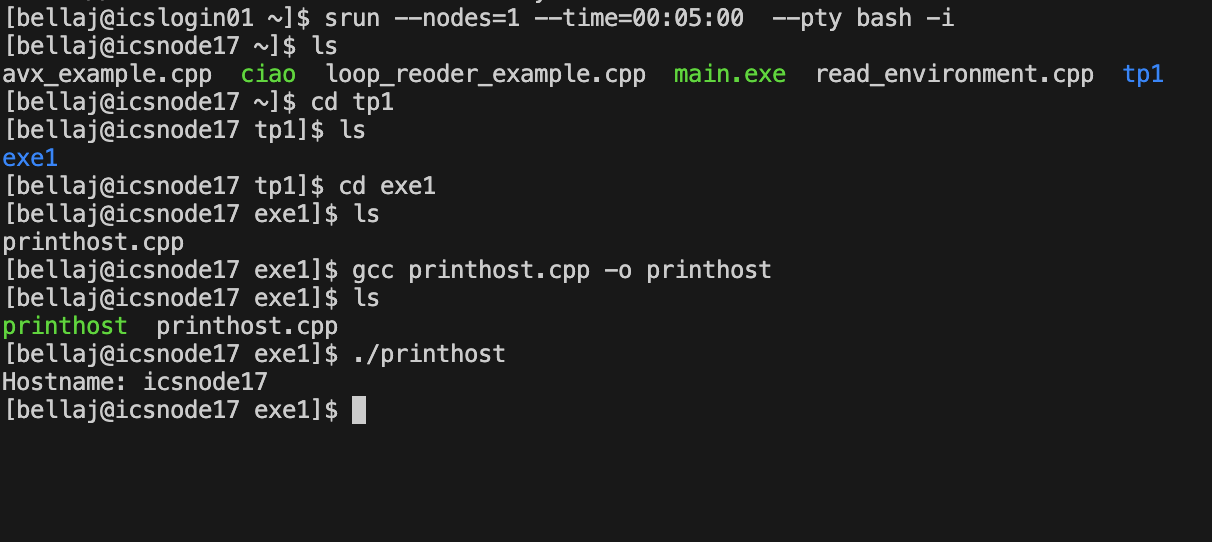
\includegraphics[width=0.7\textwidth]{./exercise1/exe1-3.png}
    \caption{Terminal of Cluster print while testing the code}
\end{figure}
\item Here i implemented the batch command in the file $printhostbatch.sh$ and the output is saved in the file $printhostbatch.txt$.
Notice that in the instructions is recommended to use the --constraint option to specify an available feature, however the available features are not set $"(null)"$. 
Therefore, i use the --partition option to specify the partition to run the job as an example.
\begin{figure}[h]
    \centering
    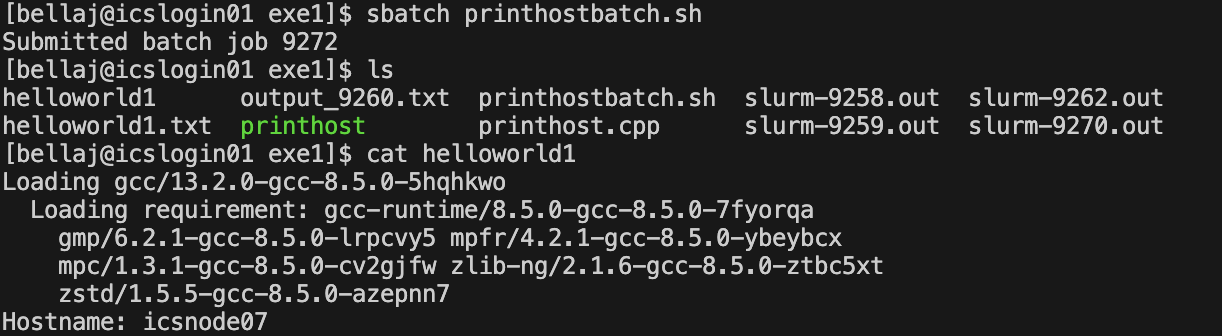
\includegraphics[width=0.7\textwidth]{./exercise1/exe14-1.png}
    \caption{Terminal of Cluster print while testing the code}
\end{figure}
\item The file $printhostbatch2node.sh$ contain the implementation of the batch script that runs the program on two nodes as requested:
\begin{figure}[h]
    \centering
    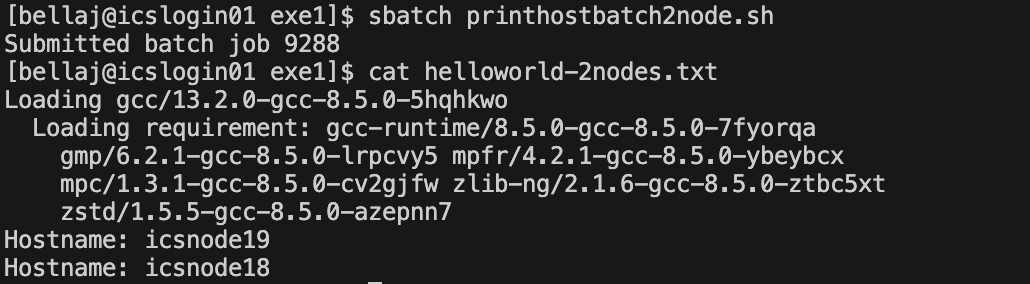
\includegraphics[width=0.7\textwidth]{./exercise1/exe15.png}
    \caption{Terminal of Cluster print while testing the code}
\end{figure}

As in previous exercises, the sources utilized are cited in the file. \footnote{At the moment I started the assignment the batch files were not included, reason why the naming is different to the provided later on and i added links that i used to understand how to construct such a file to the .sh document}
\end{enumerate}

\section{Performance Characteristics \punkte{30}}
\subsection{Peak performance}
Following the example, I visit the USI Rosa cluster specifications website \footnote{\url{https://www.ci.inf.usi.ch/research/resources/}}. 
It is possible to find that each node has 2 Intel Xeon E5-2650 v3 (25M Cache, 2.3 GHz). 

Knowing this, it was possible to find the processor specification in intel's website \footnote{\url{https://ark.intel.com/content/www/us/en/ark/products/81705/intel-xeon-processor-e5-2650-v3-25m-cache-2-30-ghz.html}},
where it is shown that the processor has 10 cores, a base frequency of 2.3 GHz ($f$ = 2.30) and supports AVX2 SIMD instructions, as specified on "Instruction Set Extensions".
Since AVX2 uses 256-bit wide vector registers, which can process 4 double-precision (64-bit) numbers at once, then $n_{SIMD}$ = 4.

With respect to FMA instructions, on Chapter 15 - section 15 of Intel’s Optimization Reference Manual Volume 1, it is mentioned that Haswell microarchitectures implements FMA instructions with execution units on port 0 and 1 and 256 - bit data paths. 
"Dot product, matrix multiplication and polynomial evaluations are expected to benefit from the use of FMA, 256 - bit data path and the independent executions on two ports. The peak throughput of FMA from each processor core are 16 single-precision
and 8 double-precision results each cycle". Therefore, $n_{FMA}$ = 2. 
In addition, it also tells us that since "...the independent executions on two ports", we can expect that the number of FP operations the FPU of a core can execute in parallel within
a single clock cycle is 2 ($n_{super}$).\footnote{It is also possible to check on \url{https://uops.info/table.html}, however the results are quite extensive even after filtering by Haswell architecture and instruction set categories.}

With this information we can compute the peak performance of a single core: 

\begin{align*}
    P_{\text{core}} &= f \times n_{\text{SIMD}} \times n_{\text{FMA}} \times n_{\text{super}} \\
                    &= 2.3 \times 4 \times 2 \times 2 \\
                    &= 36.8 \text{ GFLOP/s}
\end{align*}

As i mentioned before, each processor has 10 cores, therefore each CPU has a peak performance of 368 GFLOP/s.

\begin{align*}
    P_{\text{CPU}} &= n_{\text{cores}} \times P_{\text{core}} \\
                    &= 10 \times 36.8 \text{ GFLOP/s} \\
                    &= 368 \text{ GFLOP/s}
\end{align*}

Since in the cluster website it is specified that there are two sockets per node, then the peak performance of a node is 736 GFLOP/s:

\begin{align*}
    P_{\text{node}} &= n_{\text{sockets}} \times P_{\text{CPU}} \\
                    &= 2 \times 368.0 \text{ GFLOP/s} \\
                    &= 736 \text{ GFLOP/s}
\end{align*}

Finally, it is also specified that there are 42 compute nodes in total in the cluster: 

\begin{align*}
    P_{\text{cluster}} &= n_{\text{nodes}} \times P_{\text{node}} \\
                    &= 42 \times 736.0 \text{ GFLOP/s} \\
                    &= 30.912 \text{ TFLOP/s}
\end{align*}

Which means that the peak performance of the cluster is 30.912 TFLOP/s.

\subsection{Memory Hierarchies}
I present each terminal output after following the instructions:

\begin{figure}[H]
    \centering
    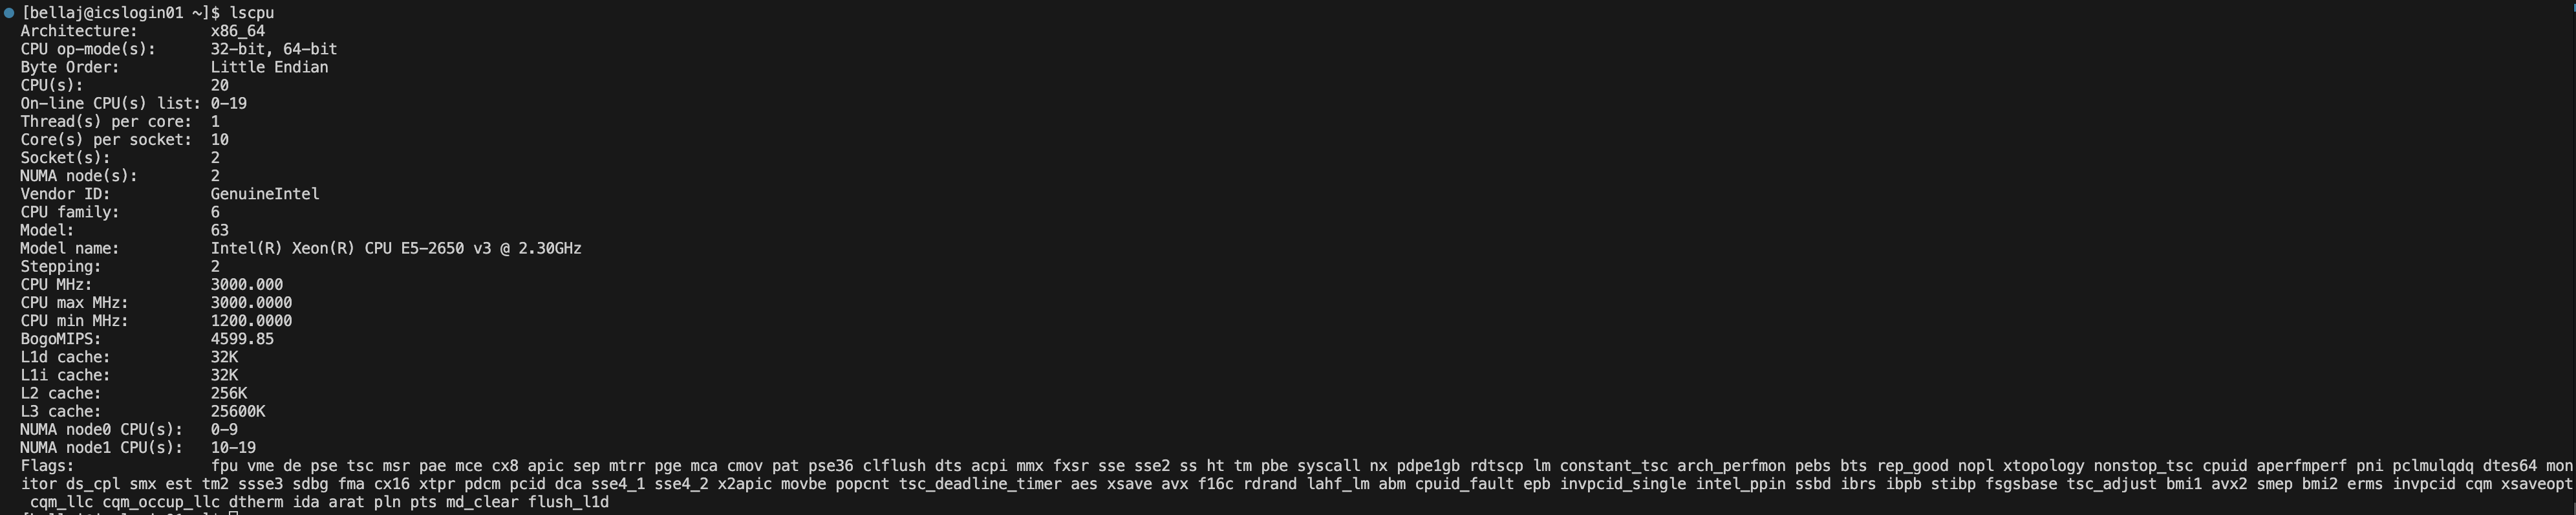
\includegraphics[width=\textwidth]{./exercise2/1.png}
    \caption{CPU model and specificiations}
  \end{figure}

Here we can observe the CPU model and specifications of the cluster. 
Which confirms the information we could obtain from the cluster website and the Intel's website.

We proceed to obtain the main memory information as indicated in the commands: 
\begin{figure}[H]
    \centering
    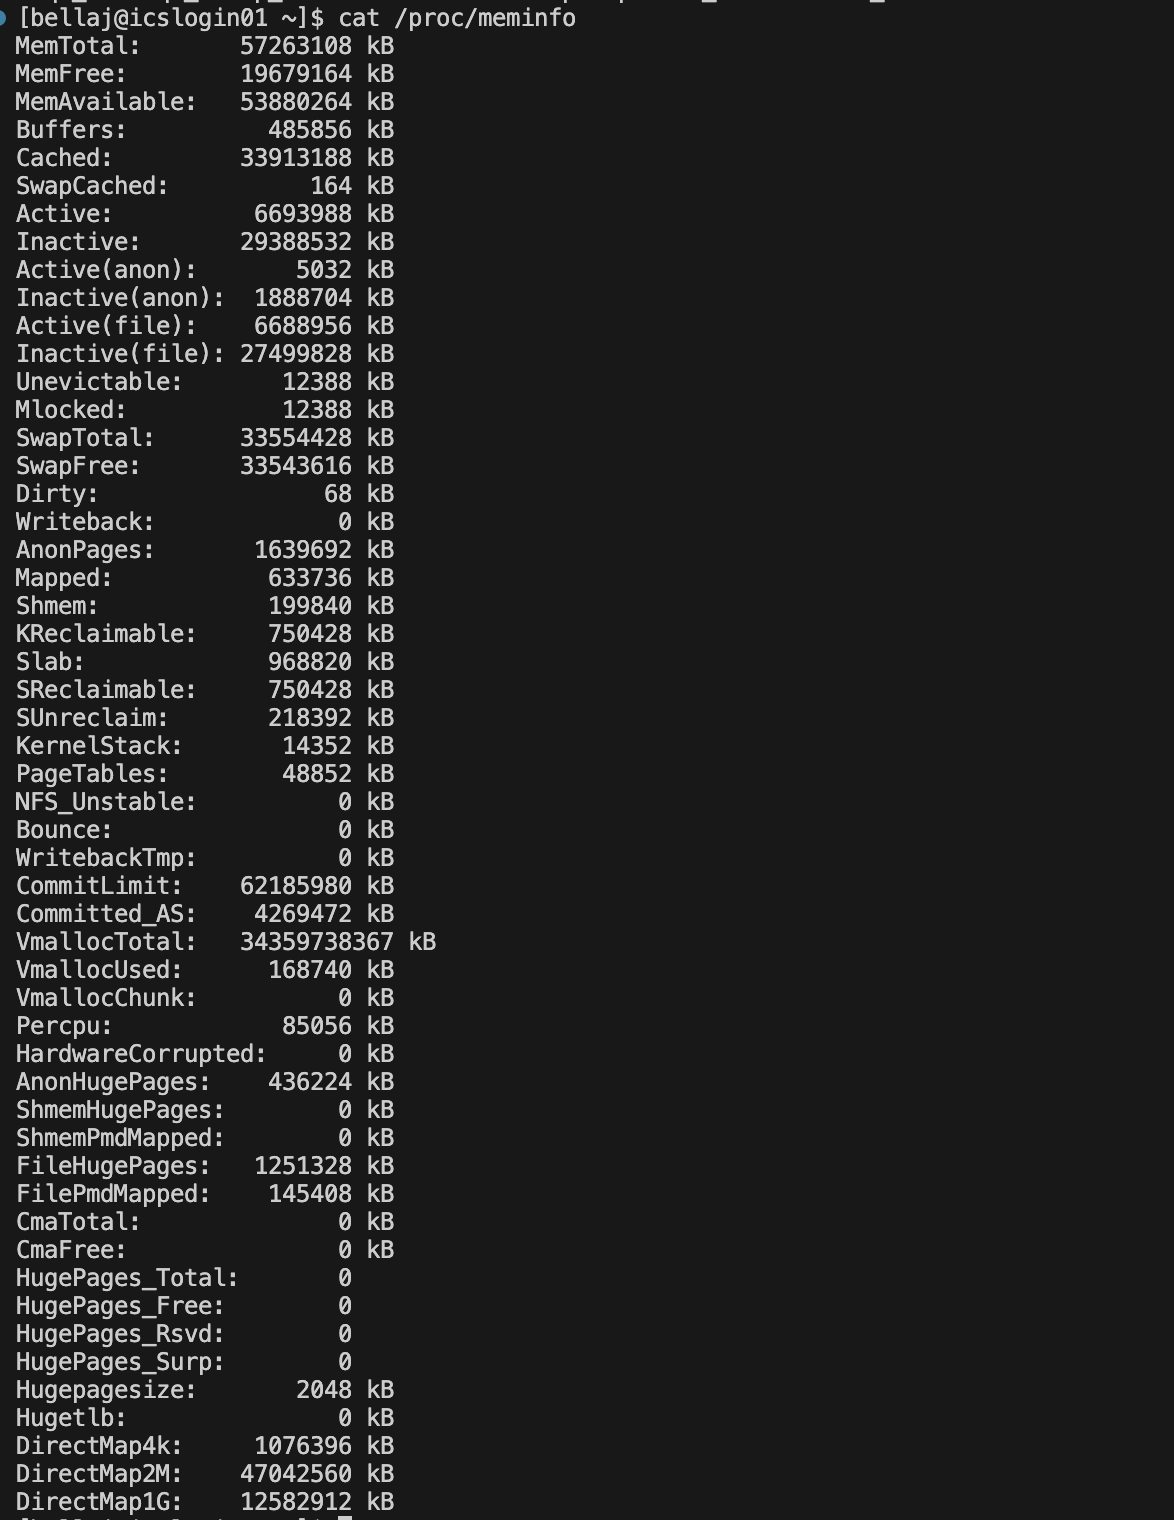
\includegraphics[width=0.6\textwidth]{./exercise2/2.png}
    \caption{Main memory information}
  \end{figure}

Now we proceed with the cache information:
\begin{figure}[H]
    \centering
    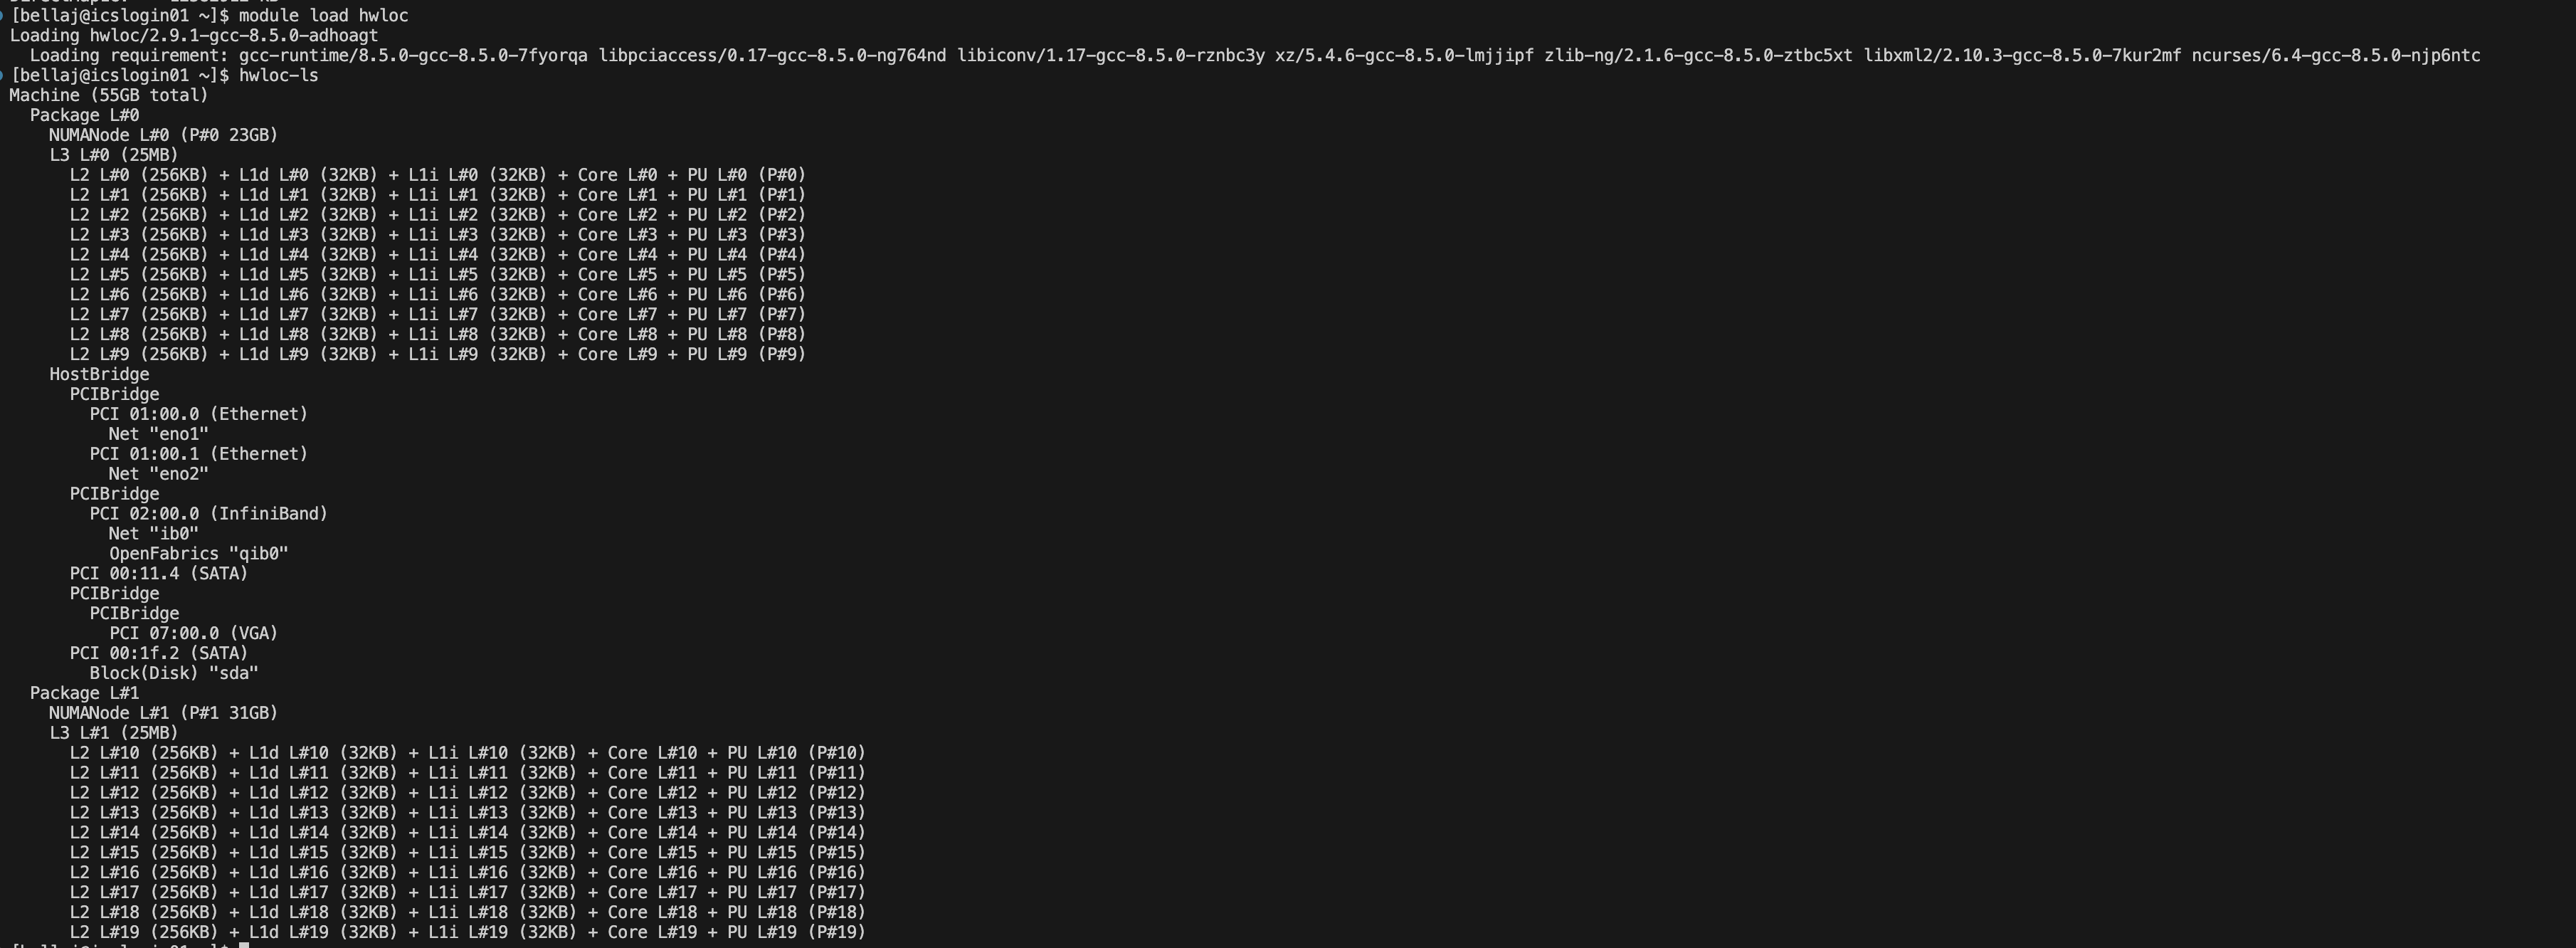
\includegraphics[width=\textwidth]{./exercise2/3.png}
    \caption{Cache memory information}
\end{figure}

Where it is possible to see that, since we are reporting about the login node, it has 55 GB of total memory, and it is composed of 2 "NUMA" nodes with 10 cores each.
Its total memory is distributed such as 23 GB of RAM memory belonging to the first package and 31 to the second one. 
Then, each package has an L3 cache memory of 25 MB each, and it is shared among all the cores each of the packages. 
The L2 cache memory has 256 KB and L1 cache memory has 32 KB (for each L1i - instruction and L1d - data) on each package too. 

This can be visualized in the downloaded figure as required:\footnote{I had troubles downloading it through the terminal with the provided command given permission issues, but I could download it through VS Code.} 

\begin{figure}[H]
    \centering
    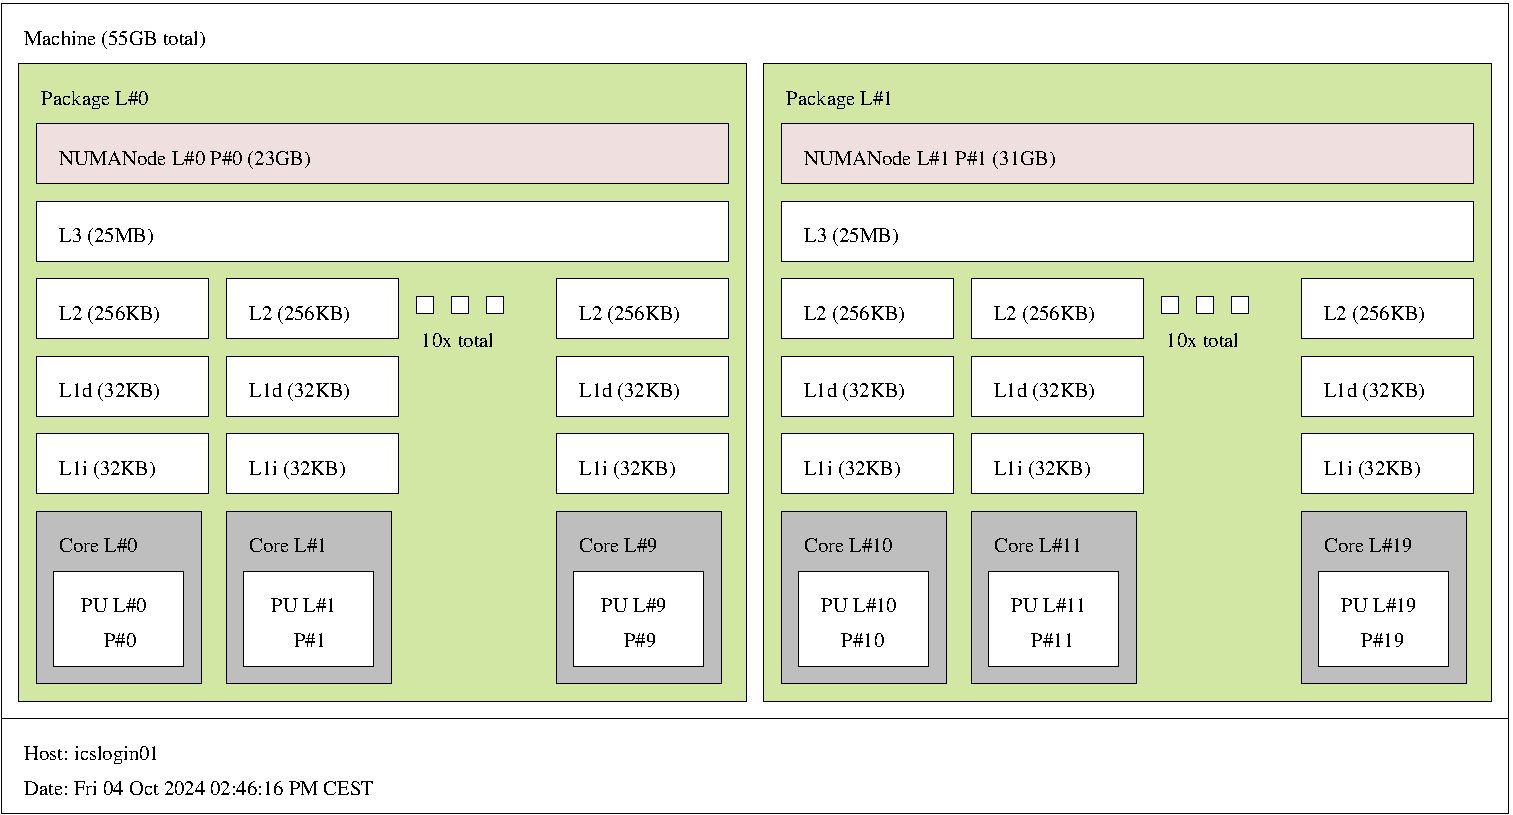
\includegraphics[width=\textwidth]{./exercise2/XEON_E5-2650.pdf}
    \caption{Resulting PDF figure from ROSA Cluster - memory Hierarchies }
  \end{figure}

\subsection{Bandwidth: STREAM benchmark}
After downloading the proper files (stream.c and mysecond.c), I proceed with the calculations required to run properly the file.
In particular, as it is mentioned in the instructions, each array must be at least four times the size of the L3 cache memory.
Therefore, since each L3 cache memory is 25 MB, then the size of each array must be at least 100 MB. 
In line 176 of the stream.c file, it is defined that the stream type is a double and since a double in C is 8 bytes (64 bits), then 100 MB / 8 = 12.5 M doubles (12500000). 
To approximate it into a power of two number, we can choose 12800000. Notice that this number is one magnitude smaller than the provided in the example, but it can be seen that both provide similar
results, since, as calculated, the size of the array is at least four times the size of the L3 cache memory in both cases.

Now, I run the commands with the specified changes: 
\begin{figure}[H]
    \centering
    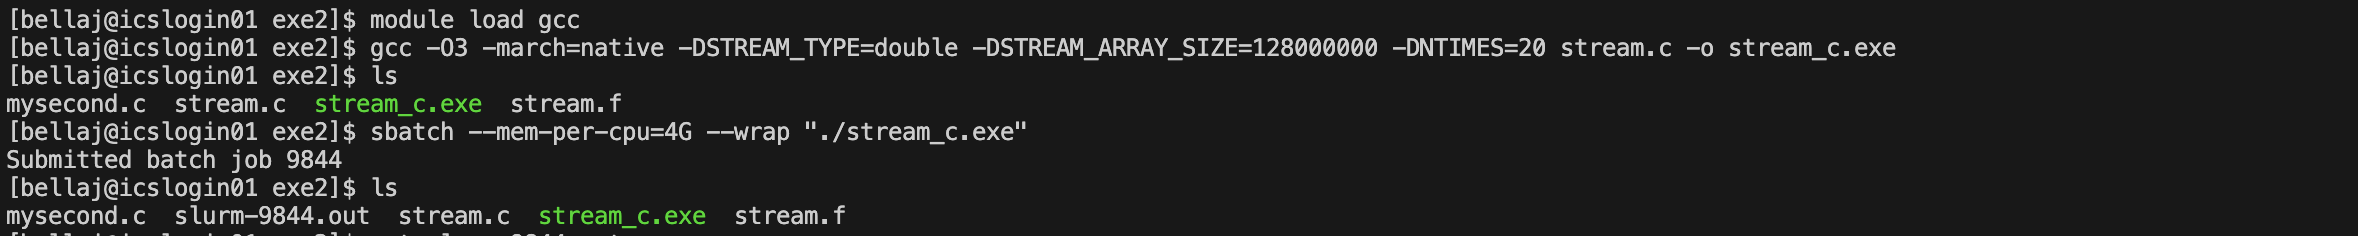
\includegraphics[width=\textwidth]{./exercise2/4.png}
    \caption{Terminal commands on ROSA cluster to obtain the STREAM benchmark - same I did with 12800000}
\end{figure}

With the resulting benchmarks as shown in the file $slurm9844.out$ and $slurm9846.out$:

\begin{figure}[H]
    \centering
    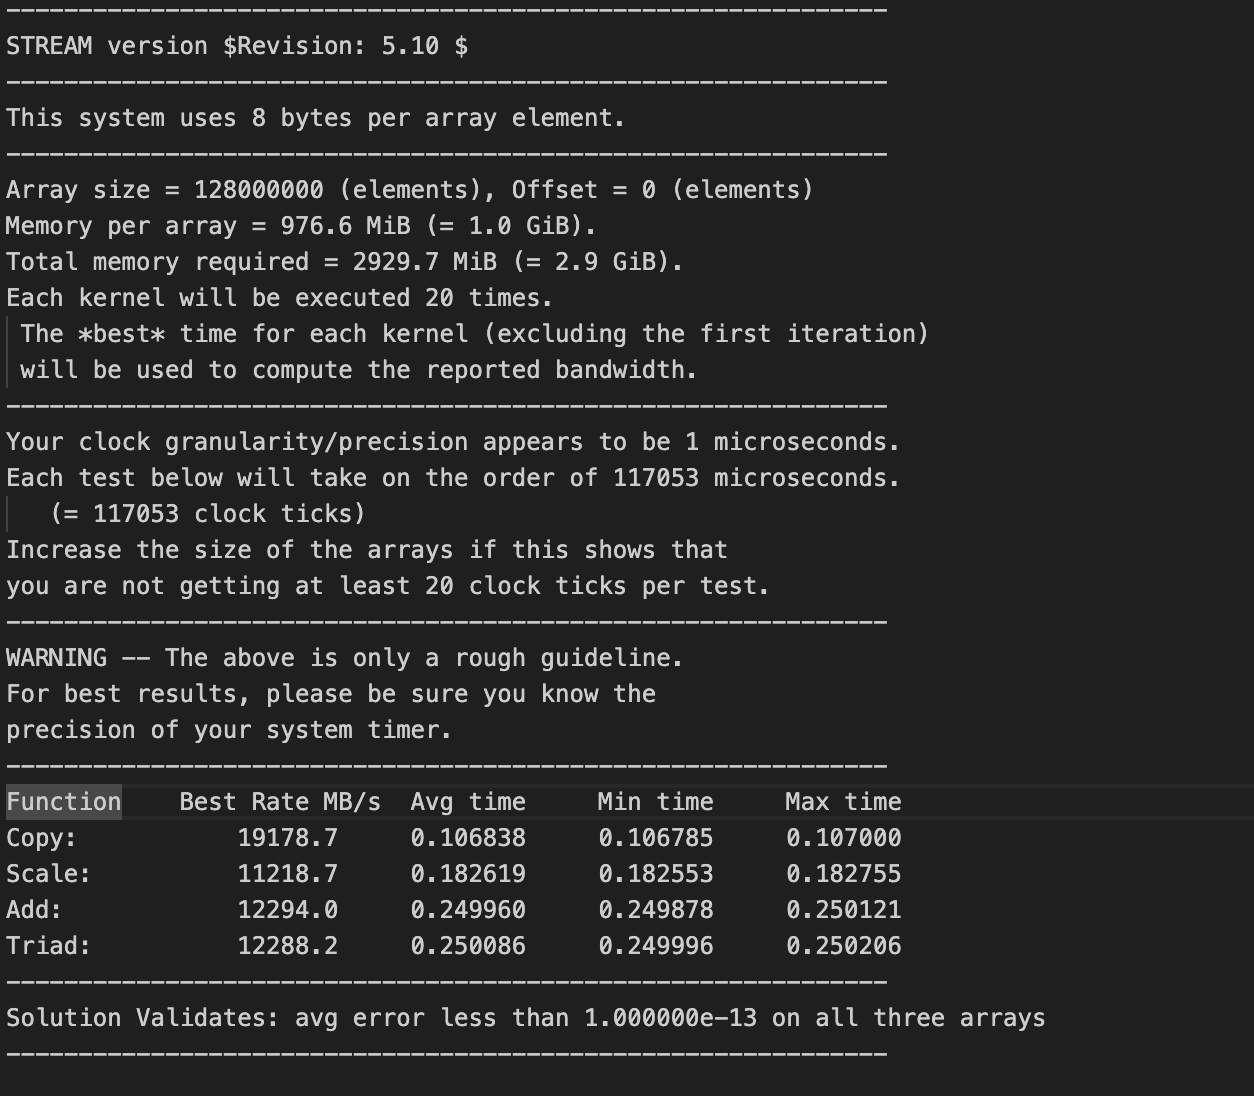
\includegraphics[width=\textwidth]{./exercise2/5.png}
    \caption{STREAM benchmark results}
\end{figure}

\begin{figure}[H]
    \centering
    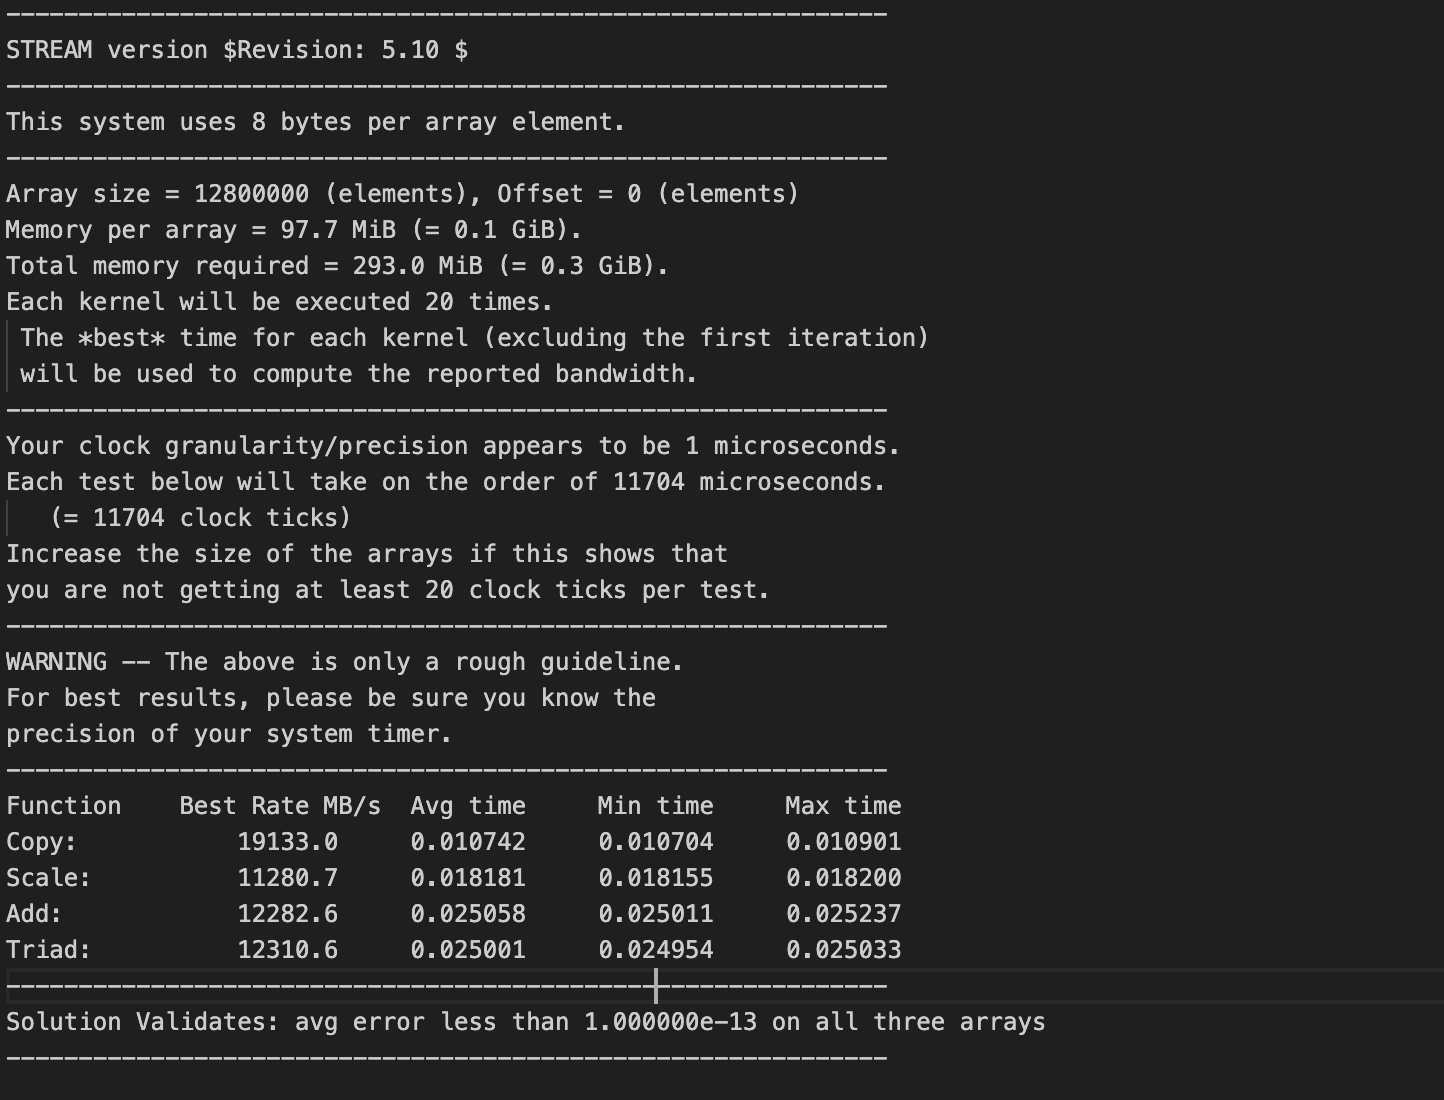
\includegraphics[width=\textwidth]{./exercise2/6.png}
    \caption{STREAM benchmark results  - with 12800000 array size as calculated} 
\end{figure}

\subsection{Performance model: A simple roofline model}
Let's put together all the information we gathered to build a simple roofline model as in the provided example. 
On one side, we know that the y-axis of the roofline model measures the attainable floating-point performance, as gigaflops per second (Giga Floating-Point Operations per Second - GFLOP/s).
On the other side, the x-axis measures the operational intensity as flops per byte of DRAM traffic \footnote{Based on Samuel Williams, Andrew Waterman, and David Patterson. Roofline: an insightful visual performance model
for multicore architectures. Communications of the ACM, 52(4):65, April 2009. \url{https://dl.acm.org/doi/10.1145/1498765.1498785} and class slide.} (the number of floating-point operations per byte of data moved from memory to the processor - Operational Intensity / [Flops/byte]).
Therefore, low operational intensity means that the system is moving a lot of data but doing little computation - memory bound. whereas high operational intensity means that the system is performing a lot of computations with the data it moves. 

As we computed in 2.1, we know that the theoretical peak performance of a core with the described characteristics in these exercises is 36.8 GFLOP/s. 
Whereas, using the same approach that in the provided example of taking the STREAM benchmark results of Scale, Add, Triad (treating Copy as an exception), we can average the results of these three:

\begin{align*}
    \text{Average maximum bandwidth} &= \frac{11280.7 + 12282.6 + 12310.6}{3} \\
                    &= 11957.97 \text{ MB/s} \\
                    &= 11.96 \text{ GB/s}
\end{align*}

Following the assignment explanation and the mentioned paper, the sloped line in the graph represents the memory bound region and by consequence, the performance there is restricted by how fast the system can move data between memory and the processor (bandwidth - slope).
Then, the machine balance is the operational intensity at which the memory bandwidth is saturated.
This is the point where the performance is limited by the memory bandwidth and the peak performance of the processor is reached, the memory bound region meets the peak performance line.
To put this into math terms since it makes it easier to understand:

\begin{align*}
    \text{Attainable GFlops/sec} = \min(&\text{Peak Floating-Point Performance},\\
    &\text{Peak Memory Bandwidth} \times \text{Operational Intensity})
\end{align*}

By consequence, on the left side of the graph, the expression summarize that the attainable performance is proportional to how fast it can transfer data from memory (bandwidth) and the FLOPs it can perform per byte of data (Operational Intensity).
Another way of seeing this is that for every additional FLOP per byte of data transfer, the performance increases by a factor equal to the memory bandwidth. 


Now, in the compute-bound region, the performance is capped by the peak core performance (independently of the data transfer)

\begin{align*}
    \text{Attainable performane (GFLOP/s) } &= \text{Peak performane (GFLOP/s) }
\end{align*}

Then, the ridge, as defined in the assignment, is the point where the two regions meet:

\begin{align*}
    \text{Peak performance (GFLOP/s)} &= \text{Peak Memory Bandwidth (GB/s)} \times \text{OI (FLOP/Byte)} \\
    36.8 \text{ GFLOP/s} &= 11.96 \text{ GB/s} \times \text{Operational Intensity (FLOP/Byte)} \\
    \text{Operational Intensity (FLOP/Byte)} &= \frac{36.8 \text{ GFLOP/s}}{11.96 \text{ GB/s}} \\
    &= 3.08 \text{ FLOP/Byte}
\end{align*}

Finally, the ridge point is at 3.08 FLOP/Byte. The following graph summarize the calculations as required: 
\footnote{The code of the plot is named $plot.py$ and the resulting plot is named $roofline\_plot.png$}

\begin{figure}[H]
    \centering
    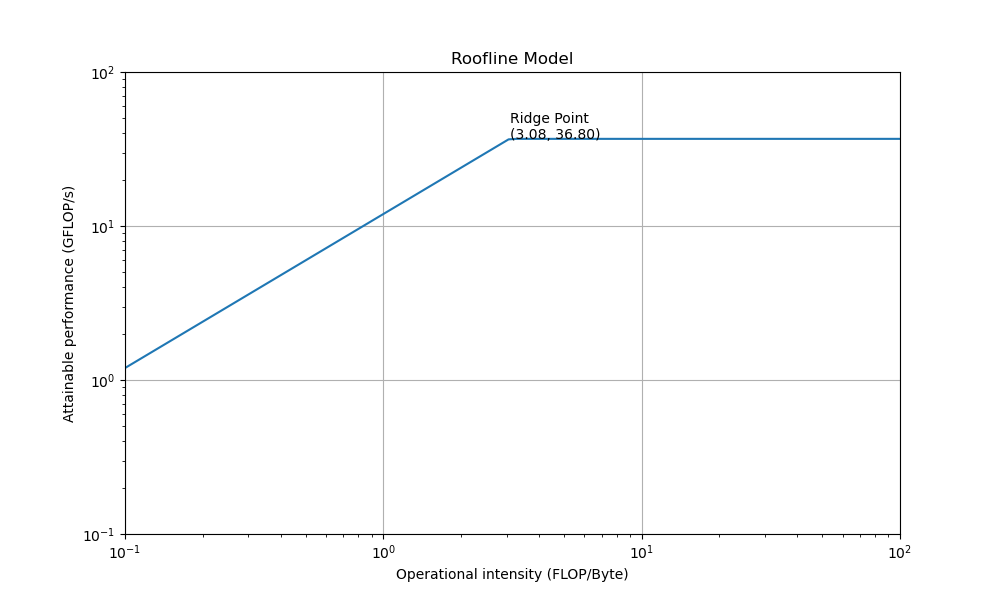
\includegraphics[width=0.85\textwidth]{./exercise2/roofline_plot.png}
    \caption{Resulting Roofline plot} 
\end{figure}
\footnote{I used python to generate the graph since, according to what I could found about graph generation in C++, 
the most common libraries used as matplotlib-cpp calls for python during compilation anyway. \url{https://stackoverflow.com/questions/63667255/plotting-graphs-in-c}}

In conclusion, given the data, kernels with operational intensity with less 3.08 FLOP/Byte will benefit the most from optimizations that improve memory access patterns or reduce memory traffic by 
restructuring loops for unit stride accesses, ensuring memory affinity, and using software prefetching. \footnote{Based on mentioned paper.}
Whereas, kernels with operational intensity with more than 3.08 FLOP/Byte could improve its computational efficiency by improving instruction-level parallelism (ILP) and applying SIMD.

\section{Optimize Square Matrix-Matrix Multiplication  \punkte{50}}
\subsection{Blocked matrix multiplication - Optimization}
To implement blocked matrix multiplication I started by computing the maximum size of each block such that it fits on the L3 cache memory. 
\footnote{I wrote the majority of my code based on the pseudocode from the last slide of HPC - "Blocked matrix multiplication", Chapter 3 of Georg Hager and Gerhard Wellein. Introduction to high performance computing for scientists and engi-
neers; and the example code provided about AVX on previous to last class.}

Since the L3 cache memory is 25 MB which is equivalent to 26214400 bytes \footnote{https://www.gbmb.org/mb-to-bytes}

Then the maximum size of each block can be calculated as $\sqrt{\frac{26214400}{3 \times 8 \text{ bytes}}}$ 
since we are working with 3 matrices (A, B, C) that are symmetric and that contains double values (8 bytes).
Therefore, the $(block\_size)^2 = (\frac{26214400}{3 \times 8 \text{ bytes}})$.

After this calculation, on the main function $square\_dgemm$, I implement the block as follows: 

First, I check if the block size is bigger than the matrix size, since in that case then we should store the matrix completely in L3 
and avoid indexing errors. Then, each of the three loops increments by calculated block size, taking into account the edge case that emerge when one of 
the loops block jumps can surpass the length of the matrix. If that occurs, the faction that computes the actual multiplication will receive the appropriate size 
of the corresponding block to not surpass the matrix size when indexing. 

Most importantly, the order of indexing follows the column-major order as specified in the assignment. Citing from the main class book \footnote{Introduction to High Performance Computing for Scientists and Engineers by Georg Hager and Gerhard Wellein, chapter 3, page 70}
"If an inner loop variable is used as an index to a multidimensional array, it should be the index that ensures stride-one access".

\begin{figure}[H]
    \centering
    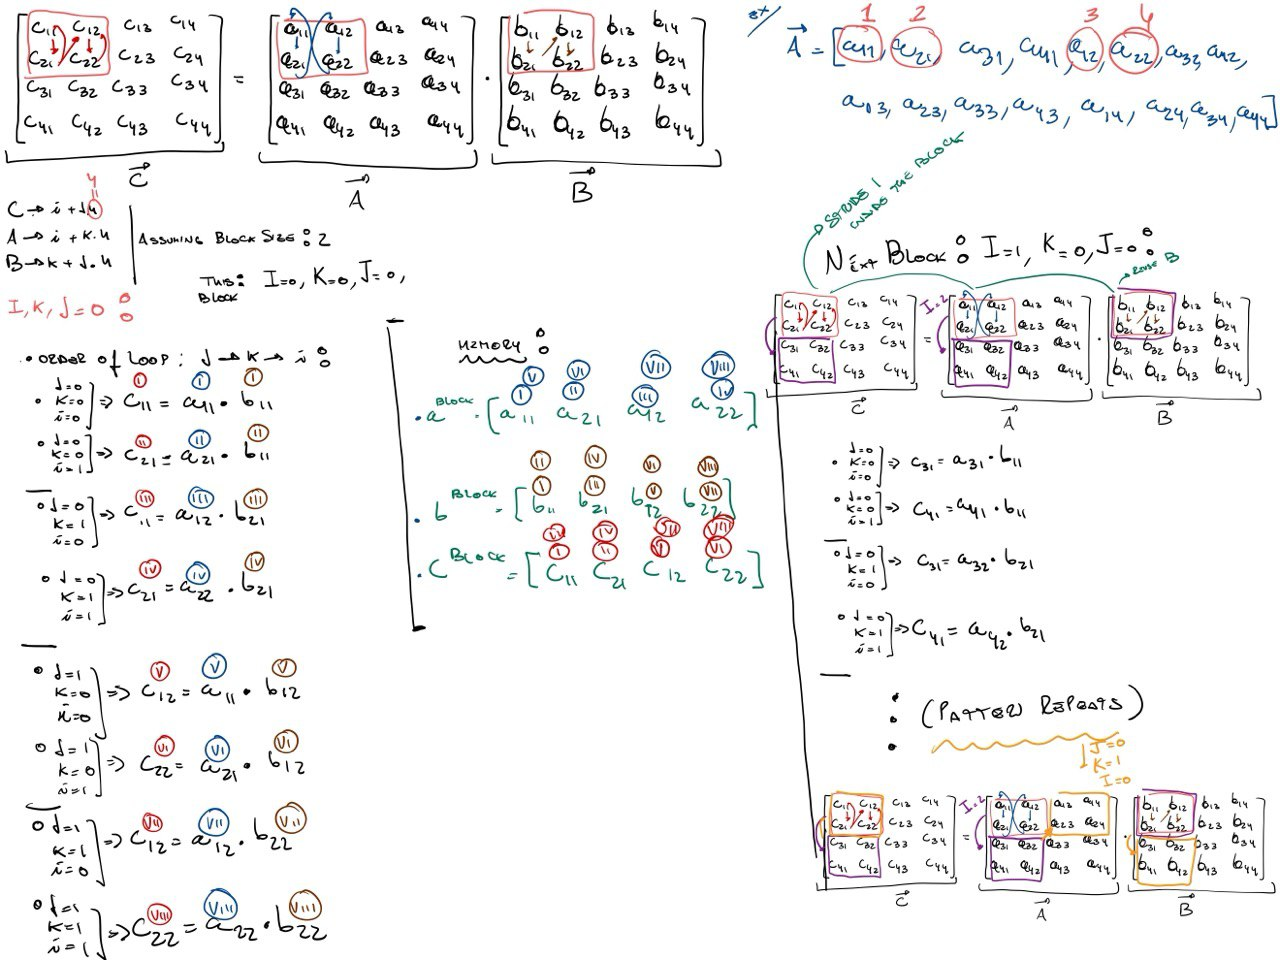
\includegraphics[width=\textwidth]{./exercise3/final-idea.jpg}
    \caption{An illustration and summary of how I thought the implementation} 
\end{figure}

Since we pass a pointer with the address of the beginning of each matrix (double* A , as we saw in previous assignment) 
then, we need to move in each block iteration the pointer to the right position of the block. 
This means, as an example, to take the first block, process it in the way I will describe below and then move the pointer to the beginning of the next block.

The block multiplication function call $matrix\_multiply\_block$ receives the matrix size, the block size of each matrix (by debugging the edge cases), and the matrices. 
Following again the column major order as described in the book, which means that if a matrix, for example, of 3x3 is store in memory as:

$[a11, a21, a31, a12, a22, a32, a13, a23, a33]$ 

To index for a particular position, we can think of "jumping" to the right column j*n and then move I step into the column row that is expected. 
However, we need to do this in a way that we can access the memory efficiently. Remembering how our matrices are stored, then we should make operations such that 
each movement is done as going down in rows into a column and then moving to the next one such that I access the C and A consecutive elements in column (stride one access)
while keeping B elements constant (same element - repeatedly) until that element will not be necessary anymore for operations. 

As we can see in my handwritten illustration (Figure 12), which shows the process that my implementation follows and its benefits over the naive implementation, 
we can see that takes into advantage two main things: 

Loading a block into cache once and reusing it multiple times - temporal locality. As it is the case with the B matrix.
And stride one access to the elements in the corresponding block of A and C - spatial locality. Iterating on each block in the column-major order.

This provided a substantial increase over the naive implementation but still far away with the provided by blas library. 

\begin{figure}[H]
    \centering
    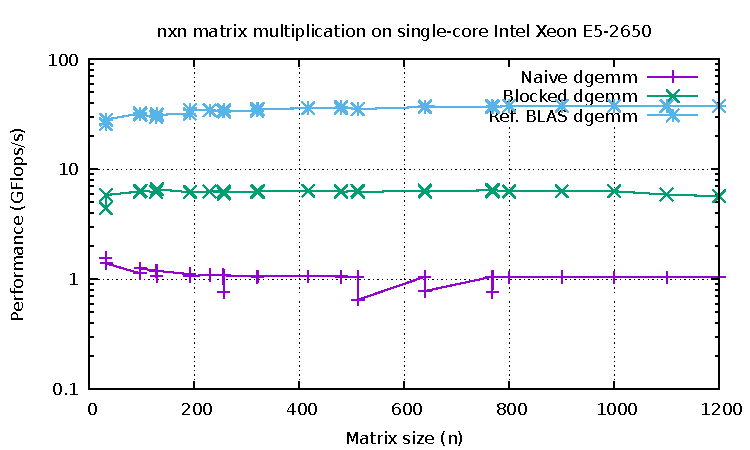
\includegraphics[width=\textwidth]{./exercise3/block/timing.pdf}
    \caption{Performance of the different implementations - Average percentage of peak performance = 16.8045} 
\end{figure}

However, there is also an additional slight improvement exist if we choose to keep fixed C block instead of B as we saw in class.
This means that the loop order of the blocks is changed to J -\> I -\> K, where K is the innermost one. Given that in my code
K index for the columns of A and J for the rows of B (as we saw in last class example, slide 44 - "$blocked\_ matrix\_multiply$"). 
Notice that for the multiplication itself, the loop order does not change since we need to keep stride one access for column-major.

\begin{figure}[H]
    \centering
    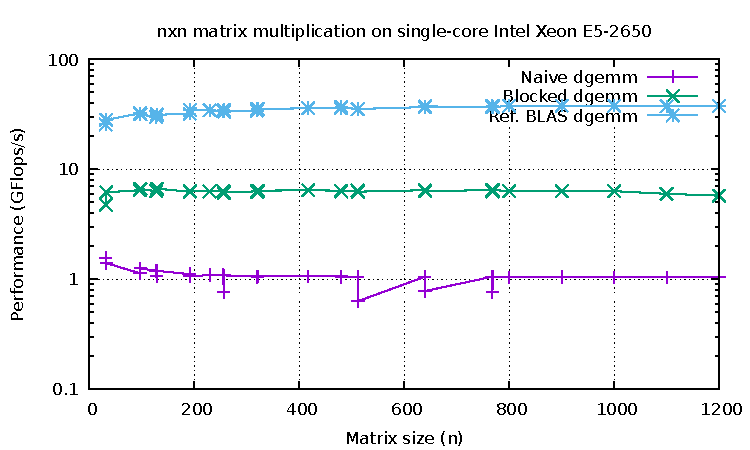
\includegraphics[width=\textwidth]{./exercise3/block-Cfixed/timing.pdf}
    \caption{Performance of the different implementations - Average percentage of peak performance = 17.0158} 
\end{figure}

The corresponding codes can be found in the folder $exercise3$, where, in $block$ folder it is the B fixed block implementation of the illustration whereas in $block\-Cfixed$ 
can be found the C fixed implementation.

\subsection{AVX optimization}
Considering these results, I tried to improve my performance by using the AVX instructions. \footnote{For this implementation i based on the following documents: 
Class code example on avx, \url{https://acl.inf.ethz.ch/teaching/fastcode/2021/slides/07-simd-avx.pdf}, and \url{http://const.me/articles/simd/simd.pdf}
}

Notice that the same illustration (Figure 12) allow us to visualize how to construct this. As i mentioned before, i constructed $square\_dgemm$ such that 
it is not necessary to modify it later on, since the later optimization can be implemented directly on the multiplication related loops, not on the blocks. 

With respect to $matrix\_multiply\_block$, the loops are almost unchanged, however, there are two main differences. 
Since we can process 4 doubles at a time with AVX (256-bits), we need to take this into account.
First, as i noted when i built the previous one, B (or C - with loop order change as in previous implementation) matrix element will be repeated until passing to the next j or k index. This pattern emerges since the independence of i
which is the inner loop. Then, we can broadcast the value of B (or C) into 4 and keeping it constant through the loop over C and A sub-blocks respectively.

The second main difference, is that we need to account for 4 loads at once in the internal loop. Which means that we loop over the index on jumps of 4. 
Which also means that we should account for the edge case where the block is not divisible by 4. This explains why I define $i$ outside I loop, such that when the 
"expected" case is finish, it keeps the value where it finishes and pass to the next loop that will manage that fragment of maximum 3 elements each in the "normal" way. 
Notice that the loading of the C and A value follows the same that in the class example of AVX. The difference here is on $\_mm256\_fmadd\_pd$, since we need to multiply A and B sub-blocks and then add the result to the C sub-block.
The function that does this, thanks to ETH slide set \footnote{https://acl.inf.ethz.ch/teaching/fastcode/2021/slides/07-simd-avx.pdf}, is the previously mentioned one. 
Finally, I store the results in the same manner as class example. 

It is finally not that exiting to report that the result was not as expected, since the implementation provided the same CPU usage as the previous one. I am still 
thinking why this could be. I suspect that in part I could be using the wrong compiling configuration: 

\begin{lstlisting}[language=bash, caption={Makefile example}]
    CC = gcc                         # compiler (& linker)
    OPT = -O3 -march=core-avx2 -mavx \
          -funroll-loops    \
          -ftree-vectorize           # optimization flags (you may add more)
    CFLAGS = -Wall -std=gnu99 $(OPT) # standard compiler flags
\end{lstlisting}
    
I tried using the commented Intel config for this, however, I keep getting an error related to not being able to 
load icx or icc. I tried to compensate this by adding the flag -mavx as it was in the AVX class example but still I do not see
any improvement, which could also mean that my AVX implementation is not correct. \footnote{To run this code, I worked in a separate
file call $dgemm\-blocked\-avx$, however, for running I copy and paste it inside the $dgemm\-blocked$ file to not modify the $run\_matrixmult.sh$.}

\begin{figure}[H]
    \centering
    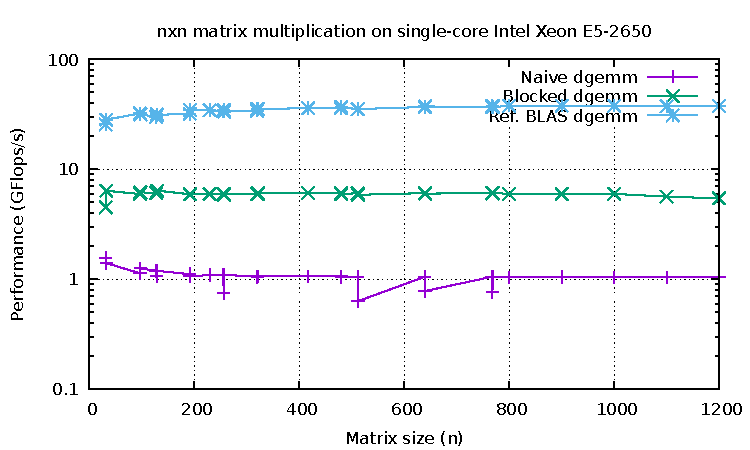
\includegraphics[width=\textwidth]{./exercise3/avx/timing-avx.pdf}
    \caption{Performance of the different implementations with AVX - Average percentage of peak performance = 16.1474} 
\end{figure}

The corresponding code can be found in the folder $exercise3$, where, in avx subfolder you will find the AVX related code whereas in block the original blocked matrix multiplication implementation.
The "$provided$" subfolder contains the rest of the code provided by the assignment.
\section{Quality of the Report  \punkte{15}}


\end{document}
